\documentclass[10pt, conference, compsocconf]{IEEEtran}

% correct bad hyphenation here
\hyphenation{op-tical net-works semi-conduc-tor}

\usepackage[pdftex]{graphicx}

\usepackage{amssymb}
\usepackage{soul}  
\usepackage[pdftex]{graphicx}
\usepackage[utf8]{inputenc} 
\usepackage{wrapfig}
\usepackage{color}
\usepackage[T1]{fontenc}
  
\begin{document}
%
% paper title
% can use linebreaks \\ within to get better formatting as desired
\title{Tool Demo: The MPS Language Workbench}

 
% author names and affiliations
% use a multiple column layout for up to two different
% affiliations

\author{\IEEEauthorblockN{Markus Voelter}
\IEEEauthorblockA{independent/itemis\\
voelter@itemis.de}
\and
\IEEEauthorblockN{Vaclav Pech}
\IEEEauthorblockA{JetBrains\\
vaclav.pech@jetbrains.com}
}

\newcommand{\changefont}[3]{\fontfamily{#1}\fontseries{#2}\fontshape{#3}\selectfont}

\newcommand\todo[1]{\mynote{TODO}{#1}} 
\newcommand{\fig}[1]{Fig.~\ref{#1}}
\newcommand{\sect}[1]{Section~\ref{#1}}
\newcommand{\ic}[1]{\changefont{cmtt}{m}{n}{#1}\normalfont}  % inline code
\newcommand{\lcr}[1]{\changefont{cmtt}{m}{n}{#1}\normalfont} % language

\newcommand{\pp}[1]{ \vspace{2mm}\noindent\textbf{{#1}} }


% make the title area
\maketitle


\begin{abstract}
JetBrains MPS is a comprehensive environment for language engineering.
It allows new languages to be defined either as standalone languages or as modular extensions of
already existing ones. Since MPS is based on using a projectional editor, syntactic forms other
than text are possible, including tables or mathematical symbols. This
demo will show MPS in the context of mbeddr C, a novel approach for embedded software
development that makes use of incremental language extension on the basis of C.
\end{abstract}

\begin{IEEEkeywords}
language engineering, language extension, language composition
\end{IEEEkeywords}

\section{Introduction and Motivation}

\noindent
Finding and working with the right abstractions for describing a
problem or its solution is one of the central pillars of software engineering. Once the right abstractions have been found, programs can be expressed more
concisely. They are easier to understand, the description can be analysed with tools and other
artifacts can be synthesized. A language is the purest form of abstraction.
It adds a suitable and convenient concrete syntax to work with the abstractions effectively. An
IDE that supports syntax coloring, code completion, error annotation and
refactoring makes working with the language and the underlying abstractions even more
productive.

Many software systems are composed of several concerns, each of which is typically expressed
with its own set of abstractions, possibly created by different people of different skills. Some of them may
not even be programmers. As a result we frequently need several languages to describe a single real-world system well.

Looking at software engineering from this perspective, clearly an environment is needed that makes
language creation easy. It should allow languages to be freely composed and the concrete
syntax should be very flexible in order to encompass the needs of all the stakeholders involved
in the software system. JetBrains MPS, an open source language workbench, is a good example of such
a system.

\section{About MPS}
 
\noindent MPS\footnote{http://jetbrains.com/mps} is an open source language
workbench, developed by JetBrains and licensed under Apache 2.0. MPS is built around the concept of a
projectional editor. This means that a wide variety of syntactic forms are supported including textual, symbolic (e.g.
mathematical), tabular and, in the upcoming version 3.0, graphical (see the
decision table in \fig{screenshot}). Even for textual notations, no grammar or
parser is used, which means that language composition cannot lead to ambiguous grammars --- ambiguities have to be
resolved by the user when entering a program. IDE support is provided for all
notations. While projectional (aka structural) editors have had a bad reputation
traditionally, MPS has managed to make the editing experience very much like
traditional text editing.
 \section{About mbeddr C}

\noindent mbeddr C\footnote{http://mbeddr.com} is an extensible version of the C
programming language implemented in MPS. It is open source under the Eclipse Public License and can
be found at \ic{http://mbeddr.com}. Development teams can build their own
domain-specific extensions of C to increase productivity and reliability in embedded software development. mbeddr C comes with a couple of reusable extensions such as
interfaces, components, unit test support and state machines. It also integrates
model checking and SAT solving to support formal verification of software
systems. By extending programming languages with suitable abstractions,
verification becomes significantly simpler.  

\begin{figure}[h]  
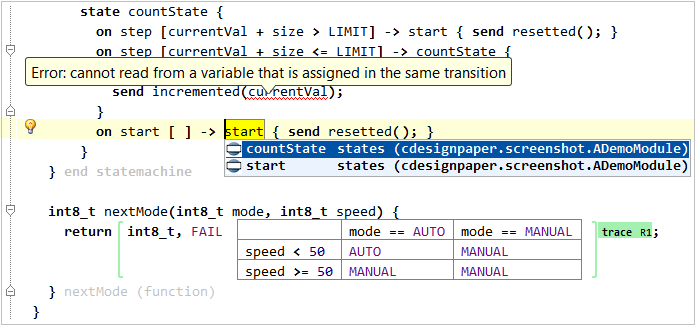
\includegraphics[width=8.6cm]{figures/screenshot.png}
\caption{An example of a program written with mbeddr C in MPS. It mixes C
functions, state machines and decision tables, each of which is defined as a separate
language. The screenshot also shows requirements traces (green annotations),
which can be attached to any program element. The definition of this language
element doesn't need to be made aware of the annotation by its creators.}
\label{screenshot}
\end{figure}

\section{Contents of the Tool Demo}

\pp{Introduction} We will introduce the need for language engineering in
the same way as in the introduction above. 

\pp{Example Use Case} We will then show an example from the mbeddr.com
extensible C language. The project develops modular extensions of
C to make embedded software development more productive. The project
demonstrates an intriguing use case for language extension and showcases
syntactic forms other than text, such as the decision table shown in FIGURE REFERENCE MISSING HERE.

\pp{Creating Extensions} The main part of the presentation will consist of a demo of how to build a language extension. Depending on the time we get for the tool demonstration, we will build the Hello World of language extensions, the \ic{unless} statement. It is basically a negated \ic{if}. This extension involves the following steps:

\begin{itemize}
  \item Defining a new language that extends C so we can "plug into" C's
  statements
  \item Defining a new concept \ic{UnlessStatement} that extends C's
  \ic{Statement} and has an \ic{Expression} and a \ic{StatementList} as children
  \item Creating an editor that projects the \ic{UnlessStatement} in the same
  way as the \ic{if}, with the keyword \ic{unless} instead
  \item Defining a type system equation that ensures the expression in the
  \ic{UnlessStatement} is Boolean
  \item Implementing a generator that maps the \ic{unless} back to an \ic{if}
  with a negated condition, so it can be compiled with a regular C compiler
  \item Defining dataflow so that MPS can detect problems such as unreachable statements or potential null references
  \item And finally, a quick fix that allows the in place transformation of
  existing \ic{if} statements to an \ic{unless} (if they don't have \ic{else
  if} or \ic{else} clauses).
\end{itemize}
This language extension shows most of the essential ingredients to language
definition in MPS.

\section{What the audience will take away}
The audience will understand the benefits of language extension. They will
realize that, with the right tools, the efforts for defining extensions is
not big, and can be easily acceptable for many real-world software development projects.

\section{Further Reading}
More details about the mbeddr approach and the capabilities of MPS can be found
in the technical report at \ic{http://bit.ly/wIYERh}.

% For peer review papers, you can put extra information on the cover
% page as needed:
% \ifCLASSOPTIONpeerreview
% \begin{center} \bfseries EDICS Category: 3-BBND \end{center}
% \fi
%
% For peerreview papers, this IEEEtran command inserts a page break and
% creates the second title. It will be ignored for other modes.
\IEEEpeerreviewmaketitle




% conference papers do not normally have an appendix





% trigger a \newpage just before the given reference
% number - used to balance the columns on the last page
% adjust value as needed - may need to be readjusted if
% the document is modified later
%\IEEEtriggeratref{8}
% The "triggered" command can be changed if desired:
%\IEEEtriggercmd{\enlargethispage{-5in}}

% references section

% can use a bibliography generated by BibTeX as a .bbl file
% BibTeX documentation can be easily obtained at:
% http://www.ctan.org/tex-archive/biblio/bibtex/contrib/doc/
% The IEEEtran BibTeX style support page is at:
% http://www.michaelshell.org/tex/ieeetran/bibtex/
%\bibliographystyle{IEEEtran}
% argument is your BibTeX string definitions and bibliography database(s)
%\bibliography{IEEEabrv,../bib/paper}
%
% <OR> manually copy in the resultant .bbl file
% set second argument of \begin to the number of references
% (used to reserve space for the reference number labels box)






% that's all folks
\end{document}


